\documentclass[]{article}
\usepackage[]{amsmath,amssymb}
\usepackage{longtable}             % tables longer than one page - used for nomenclature
\usepackage{graphicx}    % needed for including graphics e.g. EPS, PS\begin{document}
\usepackage{hyperref}
\hypersetup{
    colorlinks=true,
    linkcolor=blue,
    filecolor=magenta,      
    urlcolor=cyan,
}

\begin{document}

\section{Wishlist}
The purpose of this wishlist is to collect ideas on the implementation of usefull features in ACHP.

\subsection{Frontend//GUI}
\subsubsection{Display of the length of the different sections of the evaporator}
It would be nice to have a graph illustrating the length of the different sections
(subcooled, two-phase, superheated) of evaporator and condenser. Ideally it would be possible
to have 2 or 3 runs with different parameters plot into it to illustrate the influence
of e.g. an increase of charge.
  
\begin{figure}[htbp]
	\centering
		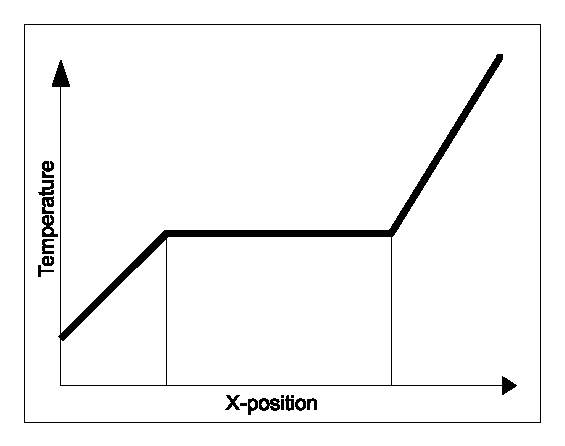
\includegraphics{wishlist_drawings_section_graph.eps}
	\label{fig:wishlist_drawings_section_graph}
	\caption{Graph showing sections of the evaporator}
\end{figure}


\subsection{Backend}
\begin{itemize}
\item The current circuitry complexity assumption is neglected. It is wished to include the effect of different circuitry configuration on the performance of heat exchanger.
\item The assumption of laminar flow and internal roughness of zero is used for the calculation of friction factor in the single phase flow (\href{https://github.com/bo3mrh/ACHP-1/blob/master/ACHP/Correlations.py#L477}{Refrence}). Therefore, it is desired to create a library with all different materials and their corresponding roughness, and the user have the option to pick the material for each component as an input. Otherwise, the default material, for example Copper, will be selected.
\end{itemize}

\end{document}
